% Options for packages loaded elsewhere
\PassOptionsToPackage{unicode}{hyperref}
\PassOptionsToPackage{hyphens}{url}
%
\documentclass[
]{article}
\usepackage{amsmath,amssymb}
\usepackage{lmodern}
\usepackage{iftex}
\ifPDFTeX
  \usepackage[T1]{fontenc}
  \usepackage[utf8]{inputenc}
  \usepackage{textcomp} % provide euro and other symbols
\else % if luatex or xetex
  \usepackage{unicode-math}
  \defaultfontfeatures{Scale=MatchLowercase}
  \defaultfontfeatures[\rmfamily]{Ligatures=TeX,Scale=1}
\fi
% Use upquote if available, for straight quotes in verbatim environments
\IfFileExists{upquote.sty}{\usepackage{upquote}}{}
\IfFileExists{microtype.sty}{% use microtype if available
  \usepackage[]{microtype}
  \UseMicrotypeSet[protrusion]{basicmath} % disable protrusion for tt fonts
}{}
\makeatletter
\@ifundefined{KOMAClassName}{% if non-KOMA class
  \IfFileExists{parskip.sty}{%
    \usepackage{parskip}
  }{% else
    \setlength{\parindent}{0pt}
    \setlength{\parskip}{6pt plus 2pt minus 1pt}}
}{% if KOMA class
  \KOMAoptions{parskip=half}}
\makeatother
\usepackage{xcolor}
\usepackage[margin=1in]{geometry}
\usepackage{color}
\usepackage{fancyvrb}
\newcommand{\VerbBar}{|}
\newcommand{\VERB}{\Verb[commandchars=\\\{\}]}
\DefineVerbatimEnvironment{Highlighting}{Verbatim}{commandchars=\\\{\}}
% Add ',fontsize=\small' for more characters per line
\usepackage{framed}
\definecolor{shadecolor}{RGB}{248,248,248}
\newenvironment{Shaded}{\begin{snugshade}}{\end{snugshade}}
\newcommand{\AlertTok}[1]{\textcolor[rgb]{0.94,0.16,0.16}{#1}}
\newcommand{\AnnotationTok}[1]{\textcolor[rgb]{0.56,0.35,0.01}{\textbf{\textit{#1}}}}
\newcommand{\AttributeTok}[1]{\textcolor[rgb]{0.77,0.63,0.00}{#1}}
\newcommand{\BaseNTok}[1]{\textcolor[rgb]{0.00,0.00,0.81}{#1}}
\newcommand{\BuiltInTok}[1]{#1}
\newcommand{\CharTok}[1]{\textcolor[rgb]{0.31,0.60,0.02}{#1}}
\newcommand{\CommentTok}[1]{\textcolor[rgb]{0.56,0.35,0.01}{\textit{#1}}}
\newcommand{\CommentVarTok}[1]{\textcolor[rgb]{0.56,0.35,0.01}{\textbf{\textit{#1}}}}
\newcommand{\ConstantTok}[1]{\textcolor[rgb]{0.00,0.00,0.00}{#1}}
\newcommand{\ControlFlowTok}[1]{\textcolor[rgb]{0.13,0.29,0.53}{\textbf{#1}}}
\newcommand{\DataTypeTok}[1]{\textcolor[rgb]{0.13,0.29,0.53}{#1}}
\newcommand{\DecValTok}[1]{\textcolor[rgb]{0.00,0.00,0.81}{#1}}
\newcommand{\DocumentationTok}[1]{\textcolor[rgb]{0.56,0.35,0.01}{\textbf{\textit{#1}}}}
\newcommand{\ErrorTok}[1]{\textcolor[rgb]{0.64,0.00,0.00}{\textbf{#1}}}
\newcommand{\ExtensionTok}[1]{#1}
\newcommand{\FloatTok}[1]{\textcolor[rgb]{0.00,0.00,0.81}{#1}}
\newcommand{\FunctionTok}[1]{\textcolor[rgb]{0.00,0.00,0.00}{#1}}
\newcommand{\ImportTok}[1]{#1}
\newcommand{\InformationTok}[1]{\textcolor[rgb]{0.56,0.35,0.01}{\textbf{\textit{#1}}}}
\newcommand{\KeywordTok}[1]{\textcolor[rgb]{0.13,0.29,0.53}{\textbf{#1}}}
\newcommand{\NormalTok}[1]{#1}
\newcommand{\OperatorTok}[1]{\textcolor[rgb]{0.81,0.36,0.00}{\textbf{#1}}}
\newcommand{\OtherTok}[1]{\textcolor[rgb]{0.56,0.35,0.01}{#1}}
\newcommand{\PreprocessorTok}[1]{\textcolor[rgb]{0.56,0.35,0.01}{\textit{#1}}}
\newcommand{\RegionMarkerTok}[1]{#1}
\newcommand{\SpecialCharTok}[1]{\textcolor[rgb]{0.00,0.00,0.00}{#1}}
\newcommand{\SpecialStringTok}[1]{\textcolor[rgb]{0.31,0.60,0.02}{#1}}
\newcommand{\StringTok}[1]{\textcolor[rgb]{0.31,0.60,0.02}{#1}}
\newcommand{\VariableTok}[1]{\textcolor[rgb]{0.00,0.00,0.00}{#1}}
\newcommand{\VerbatimStringTok}[1]{\textcolor[rgb]{0.31,0.60,0.02}{#1}}
\newcommand{\WarningTok}[1]{\textcolor[rgb]{0.56,0.35,0.01}{\textbf{\textit{#1}}}}
\usepackage{graphicx}
\makeatletter
\def\maxwidth{\ifdim\Gin@nat@width>\linewidth\linewidth\else\Gin@nat@width\fi}
\def\maxheight{\ifdim\Gin@nat@height>\textheight\textheight\else\Gin@nat@height\fi}
\makeatother
% Scale images if necessary, so that they will not overflow the page
% margins by default, and it is still possible to overwrite the defaults
% using explicit options in \includegraphics[width, height, ...]{}
\setkeys{Gin}{width=\maxwidth,height=\maxheight,keepaspectratio}
% Set default figure placement to htbp
\makeatletter
\def\fps@figure{htbp}
\makeatother
\setlength{\emergencystretch}{3em} % prevent overfull lines
\providecommand{\tightlist}{%
  \setlength{\itemsep}{0pt}\setlength{\parskip}{0pt}}
\setcounter{secnumdepth}{-\maxdimen} % remove section numbering
\ifLuaTeX
  \usepackage{selnolig}  % disable illegal ligatures
\fi
\IfFileExists{bookmark.sty}{\usepackage{bookmark}}{\usepackage{hyperref}}
\IfFileExists{xurl.sty}{\usepackage{xurl}}{} % add URL line breaks if available
\urlstyle{same} % disable monospaced font for URLs
\hypersetup{
  pdftitle={Rmarkdown exercise},
  pdfauthor={Pol},
  hidelinks,
  pdfcreator={LaTeX via pandoc}}

\title{Rmarkdown exercise}
\author{Pol}
\date{2023-05-08}

\begin{document}
\maketitle

\hypertarget{available-books-links}{%
\section{Available books links}\label{available-books-links}}

\href{intro2r.com}{Intro2R}

\href{https://bookdown.org/yihui/rmarkdown/}{Rmarkdown, the definitive
guide}

\hypertarget{rmarkdown-exercise}{%
\section{Rmarkdown exercise}\label{rmarkdown-exercise}}

\hypertarget{packages-for-rmarkdown}{%
\paragraph{Packages for Rmarkdown}\label{packages-for-rmarkdown}}

\begin{Shaded}
\begin{Highlighting}[]
\FunctionTok{install.packages}\NormalTok{(}\StringTok{"rmarkdown"}\NormalTok{)}
\FunctionTok{install.packages}\NormalTok{(}\StringTok{"tinytex"}\NormalTok{)}
\NormalTok{tinytex}\SpecialCharTok{::}\FunctionTok{install\_tinytex}\NormalTok{() }\CommentTok{\# Tinytex is requred for PDF format}
\FunctionTok{library}\NormalTok{(rmarkdown)}
\end{Highlighting}
\end{Shaded}

\hypertarget{create-list-and-extract-directories-and-files}{%
\paragraph{Create, list and extract directories and
files}\label{create-list-and-extract-directories-and-files}}

\begin{Shaded}
\begin{Highlighting}[]
\FunctionTok{dir.create}\NormalTok{(}\StringTok{"output"}\NormalTok{) }\CommentTok{\# Create directory}
\FunctionTok{dir.create}\NormalTok{(}\StringTok{"./output/figures"}\NormalTok{) }
\FunctionTok{unzip}\NormalTok{(}\StringTok{"all\_data.zip"}\NormalTok{) }\CommentTok{\# Unzip ZIP file}
\FunctionTok{list.files}\NormalTok{() }\CommentTok{\# List files on current directory}
\FunctionTok{list.dirs}\NormalTok{() }\CommentTok{\# List directories on current directory}
\end{Highlighting}
\end{Shaded}

\hypertarget{import-data-and-visualize-data-structure}{%
\paragraph{Import data and visualize data
structure}\label{import-data-and-visualize-data-structure}}

I am familiar with these sort of commands and I use them often on my
current PhD project. For this reason I do not go into detail.

\begin{Shaded}
\begin{Highlighting}[]
\NormalTok{pathways }\OtherTok{\textless{}{-}} \FunctionTok{read.table}\NormalTok{(}\AttributeTok{file =} \StringTok{"datasets/dataset\_overview\_pathways.txt"}\NormalTok{, }\AttributeTok{sep =} \StringTok{"}\SpecialCharTok{\textbackslash{}t}\StringTok{"}\NormalTok{, }\AttributeTok{header =}\NormalTok{ T, }\AttributeTok{stringsAsFactors =}\NormalTok{ T)}
\end{Highlighting}
\end{Shaded}

\texttt{summary()} returns some measures of central tendency of the
variables of the data set, whereas \texttt{str()} only returns the
column names and their data type.

\begin{Shaded}
\begin{Highlighting}[]
\FunctionTok{str}\NormalTok{(pathways)}
\end{Highlighting}
\end{Shaded}

\begin{verbatim}
## 'data.frame':    15 obs. of  6 variables:
##  $ X   : Factor w/ 15 levels "common_other_pways",..: 11 15 10 3 2 12 1 7 4 5 ...
##  $ OXTP: num  204 138 66 4 6 ...
##  $ DOPP: num  167 75 71 2 1 ...
##  $ SERP: num  143 71 71 2 16 ...
##  $ STEP: num  31 31 19 0 0 ...
##  $ VT.R: num  7 7 0 0 0 ...
\end{verbatim}

\begin{Shaded}
\begin{Highlighting}[]
\FunctionTok{summary}\NormalTok{(pathways)}
\end{Highlighting}
\end{Shaded}

\begin{verbatim}
##                      X          OXTP               DOPP          
##  common_other_pways   :1   Min.   :  0.0067   Min.   :  0.00605  
##  discarded_(coverage) :1   1st Qu.:  6.5000   1st Qu.:  3.00000  
##  discarded_(full STOP):1   Median :109.0000   Median : 75.00000  
##  FEL_pos_genes        :1   Mean   :137.9420   Mean   : 87.07470  
##  M7_pos_genes         :1   3rd Qu.:179.5000   3rd Qu.:128.00000  
##  mean omega_FEL       :1   Max.   :579.0000   Max.   :293.00000  
##  (Other)              :9                                         
##       SERP                STEP                VT.R       
##  Min.   :  0.00731   Min.   :  0.00000   Min.   : 0.000  
##  1st Qu.: 12.00000   1st Qu.:  0.00543   1st Qu.: 0.000  
##  Median : 68.00000   Median : 26.00000   Median : 5.000  
##  Mean   : 78.07703   Mean   : 32.08875   Mean   : 5.083  
##  3rd Qu.:107.50000   3rd Qu.: 31.00000   3rd Qu.: 7.000  
##  Max.   :256.00000   Max.   :155.00000   Max.   :20.000  
## 
\end{verbatim}

\hypertarget{rmarkdown-language}{%
\paragraph{Rmarkdown language}\label{rmarkdown-language}}

\begin{itemize}
\tightlist
\item
  \texttt{\textless{}\ Ctr\ +\ Alt\ +\ I\ \textgreater{}} opens a chunk
  of code
\item
  \texttt{echo\ =\ FALSE} can be added next to the \texttt{\{r\}} at the
  chunks of code that do not need to be shown.
\item
  \texttt{eval\ =\ FALSE} can be added next to the \texttt{\{r\}} at the
  chunks of code that do not need to be run at knitting.
\item
  Introducing images:
  \texttt{!{[}title{]}(path)\{width=???px,\ height=???px\}}
\end{itemize}

\hypertarget{create-version-control}{%
\section{Create Version Control}\label{create-version-control}}

To create a Version Control on Git, a GitHub account is required.

\hypertarget{download}{%
\subparagraph{Download}\label{download}}

Git needs to be installed in the computer. To check if it is installed,
the following can be typed in the R terminal: \texttt{git\ -\/-version}.
\href{https://git-scm.com/downloads}{Here} is the link for downloading
it.

\hypertarget{configure}{%
\subparagraph{Configure}\label{configure}}

Git in the PC

In the terminal of the computer, this needs to be typed:

\begin{verbatim}
git config --global user.email 'you@youremail.com'
git config --global user.name 'Your Name'
git config --global --list # Confirm configuration
\end{verbatim}

Git in RStudio

For RStudio to access Git:
\texttt{Tools\ \textgreater{}\ Global\ Options\ \textgreater{}\ Git/SVN\ \textgreater{}\ Git\ executable\ \textgreater{}\ \textless{}path\_to\_git\textgreater{}}

\begin{figure}
\centering
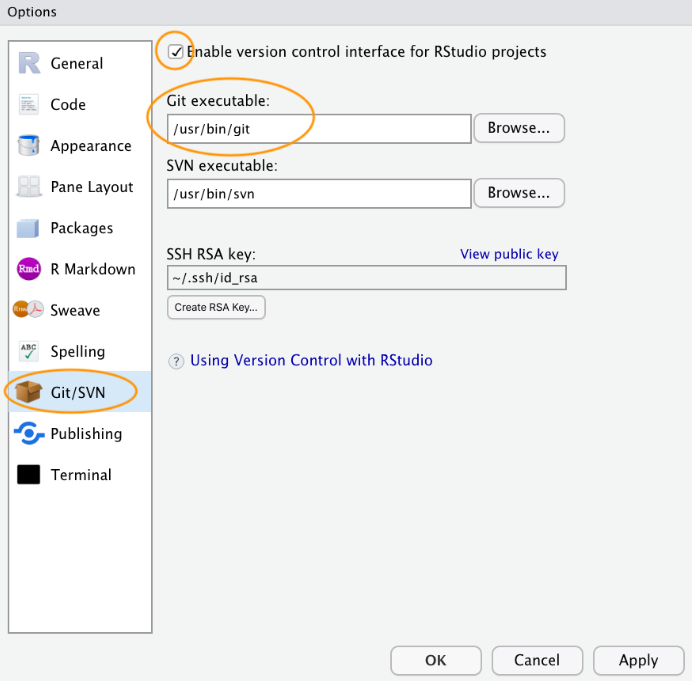
\includegraphics[width=\textwidth,height=4.16667in]{Figures/Git_in_RStudio.png}
\caption{Git in RStudio}
\end{figure}

Setting up a project in RStudio

\begin{enumerate}
\def\labelenumi{\arabic{enumi}.}
\tightlist
\item
  Create a new repository in GitHub with a README file
\item
  Create a new project with Version Control in RStudio
\end{enumerate}

\begin{itemize}
\tightlist
\item
  Include the URL of the GitHub repository
\end{itemize}

\hypertarget{using-git}{%
\subparagraph{Using Git}\label{using-git}}

Four steps on saving the changes:

\textbf{Save} in local computer (normally)

\textbf{Stage} the file in Git (brak point in the progress)

\textbf{Commit} creates a permanent snapshot of changes

\textbf{Push} to upload on GitHub

\textbf{Pull} to import from GitHub to local computer

\hypertarget{exploring-data-and-summary-statistics}{%
\section{Exploring data and summary
statistics}\label{exploring-data-and-summary-statistics}}

\hypertarget{violin-plot-nucleotide-diversity-of-all-genes}{%
\paragraph{\texorpdfstring{\textbf{Violin plot: Nucleotide Diversity of
all
genes}}{Violin plot: Nucleotide Diversity of all genes}}\label{violin-plot-nucleotide-diversity-of-all-genes}}

\begin{Shaded}
\begin{Highlighting}[]
\FunctionTok{library}\NormalTok{(}\StringTok{"ggplot2"}\NormalTok{, }\AttributeTok{verbose =}\NormalTok{ F)}
\FunctionTok{library}\NormalTok{(}\StringTok{"dplyr"}\NormalTok{, }\AttributeTok{verbose =}\NormalTok{ F)}
\CommentTok{\# Load data}
\NormalTok{pathgen }\OtherTok{\textless{}{-}} \FunctionTok{read.csv}\NormalTok{(}\StringTok{"datasets/dataset\_overview\_genes.txt"}\NormalTok{, }\AttributeTok{sep =} \StringTok{"}\SpecialCharTok{\textbackslash{}t}\StringTok{"}\NormalTok{, }\AttributeTok{header =}\NormalTok{ T)}
\CommentTok{\# Select column to plot}
\FunctionTok{colnames}\NormalTok{(pathgen)}
\end{Highlighting}
\end{Shaded}

\begin{verbatim}
## [1] "gene"             "pathway"          "source"           "nucl_div"        
## [5] "sites_FEL"        "dNdS_FEL"         "pos_site_density"
\end{verbatim}

\begin{Shaded}
\begin{Highlighting}[]
\NormalTok{column\_pl }\OtherTok{\textless{}{-}} \StringTok{"nucl\_div"}
\CommentTok{\# Group by pathway}
\NormalTok{pg\_by\_pway }\OtherTok{\textless{}{-}} \FunctionTok{group\_by}\NormalTok{(pathgen, pathway)}
\CommentTok{\# Remove NAs for the column of interest}
\NormalTok{pg\_na }\OtherTok{\textless{}{-}}\NormalTok{ pg\_by\_pway[}\SpecialCharTok{!}\NormalTok{(}\FunctionTok{is.na}\NormalTok{(}\FunctionTok{paste}\NormalTok{(}\StringTok{"dfg$"}\NormalTok{, column\_pl, }\AttributeTok{sep =} \StringTok{""}\NormalTok{))), ]}
\CommentTok{\# Violin plot variable}
\NormalTok{colors\_pways }\OtherTok{\textless{}{-}} \FunctionTok{c}\NormalTok{(}\StringTok{"STEP"} \OtherTok{=} \StringTok{"\#F8766D"}\NormalTok{, }\StringTok{"DOPP"} \OtherTok{=} \StringTok{"\#7CAE00"}\NormalTok{, }\StringTok{"VT{-}R"} \OtherTok{=} \StringTok{"\#00BFC4"}\NormalTok{, }\StringTok{"SERP"} \OtherTok{=} \StringTok{"\#C77CFF"}\NormalTok{, }\StringTok{"OXTP"} \OtherTok{=} \StringTok{"\#619CFF"}\NormalTok{) }\CommentTok{\# Assign a color to each pathway}
\NormalTok{plot\_pi }\OtherTok{\textless{}{-}} \FunctionTok{ggplot}\NormalTok{(pg\_na, }\FunctionTok{aes}\NormalTok{(}\AttributeTok{x=}\NormalTok{pathway, }\AttributeTok{y=}\NormalTok{nucl\_div, }\AttributeTok{fill=}\NormalTok{pathway)) }\SpecialCharTok{+}
  \FunctionTok{geom\_point}\NormalTok{(}\FunctionTok{aes}\NormalTok{(}\AttributeTok{color=}\NormalTok{pathway), }\AttributeTok{position=}\FunctionTok{position\_jitter}\NormalTok{(}\AttributeTok{width=}\FloatTok{0.1}\NormalTok{), }\AttributeTok{size=}\FloatTok{0.5}\NormalTok{, }\AttributeTok{alpha=}\FloatTok{0.6}\NormalTok{, }\AttributeTok{stroke =} \FloatTok{0.9}\NormalTok{, }\AttributeTok{color =} \StringTok{"black"}\NormalTok{) }\SpecialCharTok{+}
  \FunctionTok{scale\_fill\_manual}\NormalTok{(}\AttributeTok{values =}\NormalTok{ colors\_pways, ) }\SpecialCharTok{+}
  \FunctionTok{scale\_color\_manual}\NormalTok{(}\AttributeTok{values =}\NormalTok{ colors\_pways) }\SpecialCharTok{+}
  \FunctionTok{geom\_violin}\NormalTok{(}\AttributeTok{alpha =} \FloatTok{0.4}\NormalTok{, }\AttributeTok{color =} \StringTok{"transparent"}\NormalTok{)}\SpecialCharTok{+}
  \FunctionTok{geom\_text}\NormalTok{(}\AttributeTok{data =} \FunctionTok{subset}\NormalTok{(pg\_na, nucl\_div }\SpecialCharTok{\textgreater{}} \FloatTok{0.018}\NormalTok{), }\FunctionTok{aes}\NormalTok{(}\AttributeTok{label =}\NormalTok{ gene), }\AttributeTok{vjust =} \SpecialCharTok{{-}}\DecValTok{1}\NormalTok{, }\AttributeTok{size =} \DecValTok{2}\NormalTok{) }\SpecialCharTok{+} \CommentTok{\# Label filter points}
  \FunctionTok{theme\_minimal}\NormalTok{()}\SpecialCharTok{+}
  \FunctionTok{labs}\NormalTok{(}\AttributeTok{x=}\StringTok{"Pathway"}\NormalTok{, }\AttributeTok{y=}\StringTok{"index"}\SpecialCharTok{\textasciitilde{}}\NormalTok{pi}\SpecialCharTok{*}\StringTok{""}\NormalTok{)}\SpecialCharTok{+}
  \FunctionTok{ggtitle}\NormalTok{(}\StringTok{"Nucleotide diversity ("}\SpecialCharTok{\textasciitilde{}}\NormalTok{pi}\SpecialCharTok{*}\StringTok{")"}\NormalTok{)}
\CommentTok{\# Display plot}
\NormalTok{plot\_pi}
\end{Highlighting}
\end{Shaded}

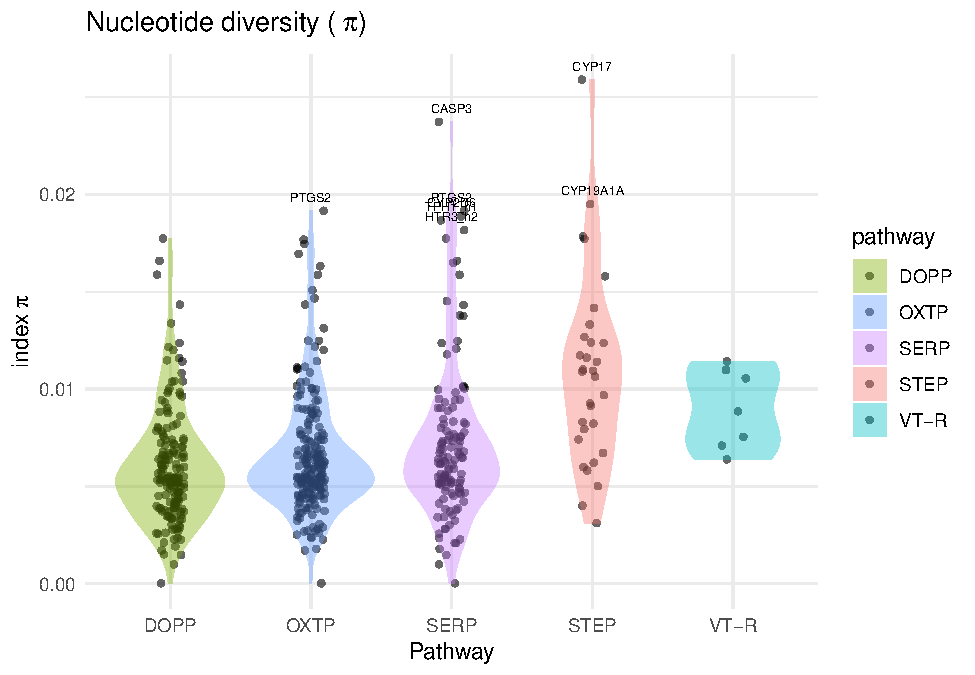
\includegraphics{RMD_file_files/figure-latex/unnamed-chunk-6-1.pdf}

\begin{Shaded}
\begin{Highlighting}[]
\CommentTok{\# Summary statistics of each pathway}
\FunctionTok{by}\NormalTok{(pg\_na}\SpecialCharTok{$}\NormalTok{nucl\_div, pg\_na}\SpecialCharTok{$}\NormalTok{pathway, summary)}
\end{Highlighting}
\end{Shaded}

\begin{verbatim}
## pg_na$pathway: DOPP
##      Min.   1st Qu.    Median      Mean   3rd Qu.      Max.      NA's 
## 0.0000262 0.0040447 0.0054190 0.0060521 0.0072740 0.0177365         3 
## ------------------------------------------------------------ 
## pg_na$pathway: OXTP
##     Min.  1st Qu.   Median     Mean  3rd Qu.     Max.     NA's 
## 0.000026 0.004832 0.005915 0.006673 0.007732 0.019159       10 
## ------------------------------------------------------------ 
## pg_na$pathway: SERP
##     Min.  1st Qu.   Median     Mean  3rd Qu.     Max.     NA's 
## 0.000026 0.004958 0.006421 0.007314 0.008397 0.023725       20 
## ------------------------------------------------------------ 
## pg_na$pathway: STEP
##     Min.  1st Qu.   Median     Mean  3rd Qu.     Max. 
## 0.003114 0.007677 0.010898 0.010863 0.012532 0.025893 
## ------------------------------------------------------------ 
## pg_na$pathway: VT-R
##     Min.  1st Qu.   Median     Mean  3rd Qu.     Max. 
## 0.006391 0.007325 0.008858 0.008978 0.010763 0.011419
\end{verbatim}

\hypertarget{lollipop-chart-top-10-genes-of-the-oxytocin-signalling-pathway}{%
\paragraph{\texorpdfstring{\textbf{Lollipop chart: Top 10 genes of the
Oxytocin Signalling
Pathway}}{Lollipop chart: Top 10 genes of the Oxytocin Signalling Pathway}}\label{lollipop-chart-top-10-genes-of-the-oxytocin-signalling-pathway}}

\begin{Shaded}
\begin{Highlighting}[]
\FunctionTok{library}\NormalTok{(}\StringTok{"ggplot2"}\NormalTok{, }\AttributeTok{verbose =}\NormalTok{ F)}
\FunctionTok{library}\NormalTok{(}\StringTok{"dplyr"}\NormalTok{, }\AttributeTok{verbose =}\NormalTok{ F)}
\NormalTok{df\_top10 }\OtherTok{\textless{}{-}} \FunctionTok{read.csv}\NormalTok{(}\StringTok{"datasets/oxtp\_FEL\_dNdS.txt"}\NormalTok{, }\AttributeTok{header =}\NormalTok{ T, }\AttributeTok{sep =} \StringTok{"}\SpecialCharTok{\textbackslash{}t}\StringTok{"}\NormalTok{)}
\CommentTok{\#Rename columns and select the ones required}
\FunctionTok{colnames}\NormalTok{(df\_top10) }\OtherTok{\textless{}{-}} \FunctionTok{c}\NormalTok{(}\StringTok{"gene"}\NormalTok{, }\StringTok{"dNdS"}\NormalTok{, }\StringTok{"pos\_sites"}\NormalTok{, }\StringTok{"total\_sites"}\NormalTok{, }\StringTok{"site\_density"}\NormalTok{)}
\NormalTok{df\_top10\_f }\OtherTok{\textless{}{-}}\NormalTok{df\_top10[}\DecValTok{1}\SpecialCharTok{:}\DecValTok{10}\NormalTok{,]}
\NormalTok{df\_top10\_f }\OtherTok{\textless{}{-}} \FunctionTok{select}\NormalTok{(df\_top10\_f, }\FunctionTok{c}\NormalTok{(gene, dNdS, site\_density))}
\NormalTok{df\_top10\_f}\SpecialCharTok{$}\NormalTok{site\_density }\OtherTok{\textless{}{-}} \FunctionTok{round}\NormalTok{(df\_top10\_f}\SpecialCharTok{$}\NormalTok{site\_density, }\FunctionTok{round}\NormalTok{(}\DecValTok{2}\NormalTok{)) }\CommentTok{\# Round to 2 decimals}

\CommentTok{\#Order by w value}
\NormalTok{df\_s }\OtherTok{\textless{}{-}}\NormalTok{ df\_top10\_f[}\FunctionTok{order}\NormalTok{(df\_top10\_f}\SpecialCharTok{$}\NormalTok{dNdS, }\AttributeTok{decreasing =}\NormalTok{ T), ]}
\NormalTok{gene\_order }\OtherTok{=} \FunctionTok{c}\NormalTok{(df\_s}\SpecialCharTok{$}\NormalTok{gene)}
\NormalTok{df\_top10\_f}\SpecialCharTok{$}\NormalTok{gene }\OtherTok{\textless{}{-}} \FunctionTok{factor}\NormalTok{(df\_top10\_f}\SpecialCharTok{$}\NormalTok{gene, }\AttributeTok{levels =} \FunctionTok{rev}\NormalTok{(gene\_order))}

\CommentTok{\#Plot}
\NormalTok{dNdS\_top10 }\OtherTok{\textless{}{-}} \FunctionTok{ggplot}\NormalTok{(df\_top10\_f, }\FunctionTok{aes}\NormalTok{(}\AttributeTok{x =}\NormalTok{ gene, }\AttributeTok{y =}\NormalTok{ dNdS)) }\SpecialCharTok{+}
  \FunctionTok{geom\_segment}\NormalTok{(}\FunctionTok{aes}\NormalTok{(}\AttributeTok{x =}\NormalTok{ gene, }\AttributeTok{xend =}\NormalTok{ gene, }\AttributeTok{y =} \FloatTok{0.2}\NormalTok{, }\AttributeTok{yend =}\NormalTok{ dNdS), }\AttributeTok{linetype=}\DecValTok{2}\NormalTok{, }\AttributeTok{color =} \StringTok{"black"}\NormalTok{, }\AttributeTok{linewidth =} \FloatTok{0.6}\NormalTok{) }\SpecialCharTok{+}
  \FunctionTok{geom\_point}\NormalTok{(}\FunctionTok{aes}\NormalTok{(}\AttributeTok{size =}\NormalTok{ site\_density), }\AttributeTok{fill =} \StringTok{"gray"}\NormalTok{, }\AttributeTok{color =} \StringTok{"black"}\NormalTok{, }\AttributeTok{shape =} \DecValTok{21}\NormalTok{, }\AttributeTok{alpha =} \DecValTok{1}\NormalTok{, }\AttributeTok{stroke =} \DecValTok{1}\NormalTok{) }\SpecialCharTok{+}
  \FunctionTok{geom\_text}\NormalTok{(}\FunctionTok{aes}\NormalTok{(}\AttributeTok{label =} \FunctionTok{paste}\NormalTok{(site\_density, }\StringTok{" \%"}\NormalTok{, }\AttributeTok{sep =} \StringTok{""}\NormalTok{)), }\AttributeTok{size =} \DecValTok{3}\NormalTok{, }\AttributeTok{color =} \StringTok{"black"}\NormalTok{, }\AttributeTok{hjust =} \SpecialCharTok{{-}}\FloatTok{0.5}\NormalTok{) }\SpecialCharTok{+}
  \FunctionTok{scale\_size}\NormalTok{(}\AttributeTok{range =} \FunctionTok{c}\NormalTok{(}\DecValTok{1}\NormalTok{, }\DecValTok{10}\NormalTok{)) }\SpecialCharTok{+}
  \FunctionTok{labs}\NormalTok{(}\AttributeTok{title =} \StringTok{"Top 10 OXTP genes dNdS ratio. "}\NormalTok{,}
       \AttributeTok{x =} \StringTok{"Gene"}\NormalTok{,}
       \AttributeTok{y =} \StringTok{"dN/dS"}\NormalTok{,}
       \AttributeTok{size =} \StringTok{"Positive sites}\SpecialCharTok{\textbackslash{}n}\StringTok{density}\SpecialCharTok{\textbackslash{}n}\StringTok{(\% of sites)"}\NormalTok{) }\SpecialCharTok{+}
  \FunctionTok{ylim}\NormalTok{(}\FloatTok{0.3}\NormalTok{, }\FloatTok{0.7}\NormalTok{) }\SpecialCharTok{+}
  \FunctionTok{theme\_minimal}\NormalTok{() }\SpecialCharTok{+}
  \FunctionTok{theme}\NormalTok{(}\AttributeTok{plot.title =} \FunctionTok{element\_text}\NormalTok{(}\AttributeTok{hjust =} \FloatTok{0.5}\NormalTok{, }\AttributeTok{size =} \DecValTok{20}\NormalTok{, }\AttributeTok{face =} \StringTok{"bold"}\NormalTok{),}
        \AttributeTok{axis.title =} \FunctionTok{element\_text}\NormalTok{(}\AttributeTok{size =} \DecValTok{12}\NormalTok{),}
        \AttributeTok{axis.text =} \FunctionTok{element\_text}\NormalTok{(}\AttributeTok{size =} \DecValTok{10}\NormalTok{),}
        \AttributeTok{legend.title =} \FunctionTok{element\_text}\NormalTok{(}\AttributeTok{size =} \DecValTok{10}\NormalTok{),}
        \AttributeTok{legend.text =} \FunctionTok{element\_text}\NormalTok{(}\AttributeTok{size =} \DecValTok{10}\NormalTok{)) }\SpecialCharTok{+} 
  \FunctionTok{coord\_flip}\NormalTok{()}

\NormalTok{dNdS\_top10}
\end{Highlighting}
\end{Shaded}

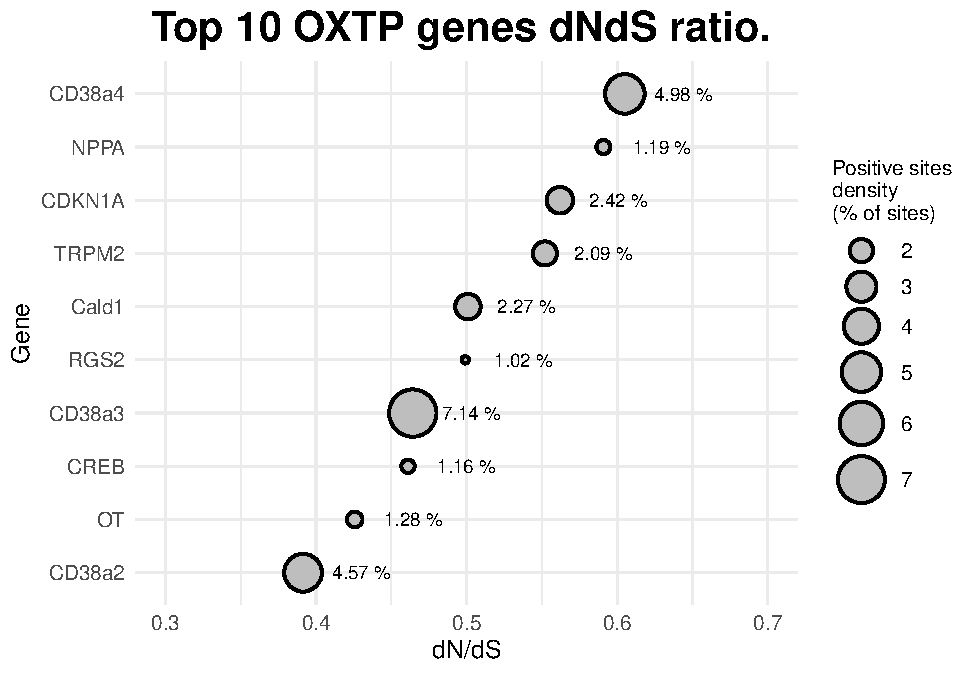
\includegraphics{RMD_file_files/figure-latex/unnamed-chunk-7-1.pdf}

\begin{Shaded}
\begin{Highlighting}[]
\CommentTok{\# Summary}
\FunctionTok{summary}\NormalTok{(df\_top10\_f)}
\end{Highlighting}
\end{Shaded}

\begin{verbatim}
##       gene        dNdS         site_density  
##  CD38a2 :1   Min.   :0.3914   Min.   :1.020  
##  OT     :1   1st Qu.:0.4619   1st Qu.:1.212  
##  CREB   :1   Median :0.5000   Median :2.180  
##  CD38a3 :1   Mean   :0.5052   Mean   :2.812  
##  RGS2   :1   3rd Qu.:0.5594   3rd Qu.:4.032  
##  Cald1  :1   Max.   :0.6050   Max.   :7.140  
##  (Other):4
\end{verbatim}

\hypertarget{scatterplot-for-discrete-variables-pair-bonding-vs-snp-refalternative}{%
\paragraph{\texorpdfstring{\textbf{Scatterplot for discrete variables:
Pair-bonding vs SNP
(ref/alternative)}}{Scatterplot for discrete variables: Pair-bonding vs SNP (ref/alternative)}}\label{scatterplot-for-discrete-variables-pair-bonding-vs-snp-refalternative}}

\begin{Shaded}
\begin{Highlighting}[]
\FunctionTok{library}\NormalTok{(}\StringTok{"ggplot2"}\NormalTok{, }\AttributeTok{verbose =}\NormalTok{ F)}
\FunctionTok{library}\NormalTok{(}\StringTok{"dplyr"}\NormalTok{, }\AttributeTok{verbose =}\NormalTok{ F)}

\NormalTok{df }\OtherTok{\textless{}{-}} \FunctionTok{read.csv}\NormalTok{(}\StringTok{"datasets/EGFR\_19907494\_PB\_BT.txt"}\NormalTok{, }\AttributeTok{sep =} \StringTok{"}\SpecialCharTok{\textbackslash{}t}\StringTok{"}\NormalTok{)}
\NormalTok{df2 }\OtherTok{\textless{}{-}} \FunctionTok{read.csv}\NormalTok{(}\StringTok{"datasets/spp{-}tribe.txt"}\NormalTok{, }\AttributeTok{sep =} \StringTok{"}\SpecialCharTok{\textbackslash{}t}\StringTok{"}\NormalTok{)}

\FunctionTok{colnames}\NormalTok{(df) }\OtherTok{\textless{}{-}} \FunctionTok{c}\NormalTok{(}\StringTok{"spp"}\NormalTok{, }\StringTok{"PB"}\NormalTok{, }\StringTok{"SNP"}\NormalTok{)}

\CommentTok{\# Merge the 2 data frames to link species and tribes}
\NormalTok{df\_final }\OtherTok{\textless{}{-}} \FunctionTok{inner\_join}\NormalTok{(df, df2, }\AttributeTok{by=}\StringTok{"spp"}\NormalTok{)}

\CommentTok{\#Plot}
\NormalTok{SNP\_vs\_PB }\OtherTok{\textless{}{-}} \FunctionTok{ggplot}\NormalTok{(df\_final, }\FunctionTok{aes}\NormalTok{(}\AttributeTok{x =}\NormalTok{ PB, }\AttributeTok{y =}\NormalTok{ SNP, }\AttributeTok{color =}\NormalTok{ tribe)) }\SpecialCharTok{+}
  \FunctionTok{geom\_point}\NormalTok{(}\AttributeTok{position=}\FunctionTok{position\_jitter}\NormalTok{(}\AttributeTok{width=}\FloatTok{0.2}\NormalTok{, }\AttributeTok{height =} \FloatTok{0.2}\NormalTok{)) }\SpecialCharTok{+}
  \FunctionTok{scale\_x\_continuous}\NormalTok{(}\AttributeTok{breaks =} \FunctionTok{c}\NormalTok{(}\DecValTok{0}\NormalTok{, }\DecValTok{1}\NormalTok{), }\AttributeTok{limits =} \FunctionTok{c}\NormalTok{(}\SpecialCharTok{{-}}\FloatTok{0.2}\NormalTok{, }\FloatTok{1.2}\NormalTok{)) }\SpecialCharTok{+}
  \FunctionTok{scale\_y\_continuous}\NormalTok{(}\AttributeTok{breaks =} \FunctionTok{c}\NormalTok{(}\DecValTok{0}\NormalTok{, }\DecValTok{1}\NormalTok{), }\AttributeTok{limits =} \FunctionTok{c}\NormalTok{(}\SpecialCharTok{{-}}\FloatTok{0.2}\NormalTok{, }\FloatTok{1.2}\NormalTok{)) }\SpecialCharTok{+}
  \FunctionTok{labs}\NormalTok{(}\AttributeTok{title =} \StringTok{"SNP allele vs phenotype (Pair{-}bonding)"}\NormalTok{,}
       \AttributeTok{x =} \StringTok{"Pair{-}bonding (0 = No ; 1 = Yes)"}\NormalTok{,}
       \AttributeTok{y =} \StringTok{"SNP (0 = Ref ; 1 = Alt)"}\NormalTok{)}

\NormalTok{SNP\_vs\_PB}
\end{Highlighting}
\end{Shaded}

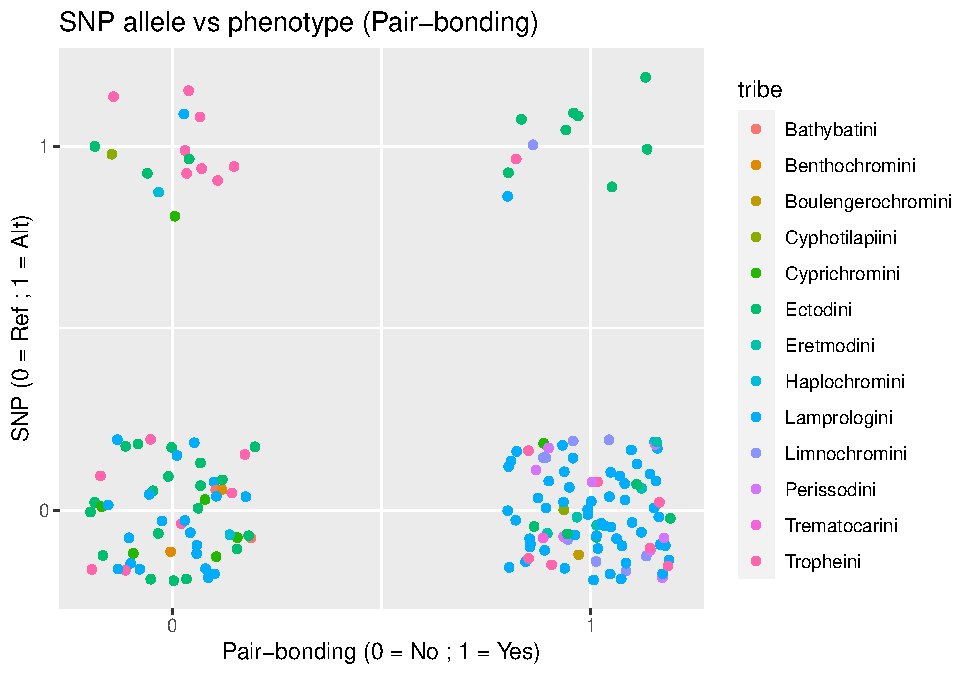
\includegraphics{RMD_file_files/figure-latex/unnamed-chunk-8-1.pdf}

\hypertarget{inferential-statistics}{%
\section{Inferential Statistics}\label{inferential-statistics}}

\hypertarget{corelation-between-nucleotide-diversity-ux3c0-and-dnds-ratio-ux3c9}{%
\paragraph{Corelation between nucleotide diversity (π) and dNdS ratio
(ω)}\label{corelation-between-nucleotide-diversity-ux3c0-and-dnds-ratio-ux3c9}}

EXPLAIN PROCESS WITH TEST FINDER

We are asking if the nucleotide diversity (index that indicates the
level of variability of a nucleotide sequences across a set of species)
is corelated with the index of positive selection (ω). By taking the
Oxytocin Signalling Pathway, we compute a Spearman's corelation test,
which does NOT assume linearity but only monotony (always same sense
-positive or negative-).

\begin{Shaded}
\begin{Highlighting}[]
\FunctionTok{library}\NormalTok{(}\StringTok{"ggplot2"}\NormalTok{, }\AttributeTok{verbose =}\NormalTok{ F)}
\FunctionTok{library}\NormalTok{(}\StringTok{"dplyr"}\NormalTok{, }\AttributeTok{verbose =}\NormalTok{ F)}
\CommentTok{\# Load data}
\NormalTok{dataset }\OtherTok{\textless{}{-}} \FunctionTok{read.csv}\NormalTok{(}\StringTok{"datasets/dataset\_overview\_genes.txt"}\NormalTok{, }\AttributeTok{sep =} \StringTok{"}\SpecialCharTok{\textbackslash{}t}\StringTok{"}\NormalTok{, }\AttributeTok{header =}\NormalTok{ T)}
\CommentTok{\# Select pathway}
\NormalTok{df\_oxtp }\OtherTok{\textless{}{-}}\NormalTok{ dataset[dataset}\SpecialCharTok{$}\NormalTok{pathway }\SpecialCharTok{==} \StringTok{"OXTP"}\NormalTok{,]}
\CommentTok{\# Plot}
\FunctionTok{ggplot}\NormalTok{(df\_oxtp, }\FunctionTok{aes}\NormalTok{(}\AttributeTok{x=}\NormalTok{nucl\_div, }\AttributeTok{y=}\NormalTok{dNdS\_FEL)) }\SpecialCharTok{+}
  \FunctionTok{geom\_point}\NormalTok{()}
\end{Highlighting}
\end{Shaded}

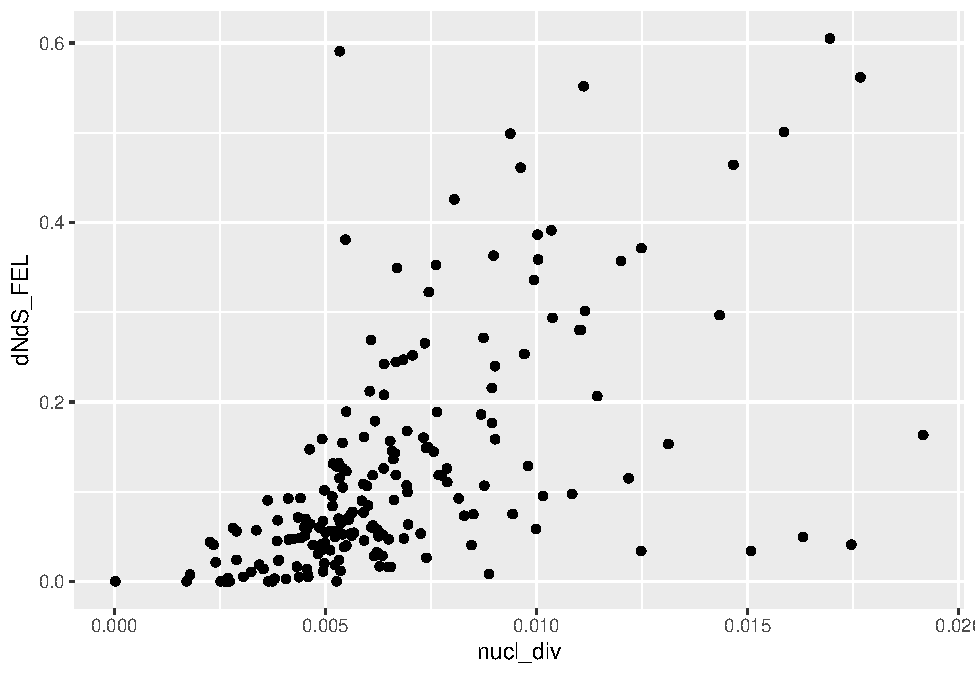
\includegraphics{RMD_file_files/figure-latex/unnamed-chunk-9-1.pdf}

\begin{Shaded}
\begin{Highlighting}[]
\CommentTok{\# Corelation}
\NormalTok{oxtp\_cor }\OtherTok{\textless{}{-}} \FunctionTok{cor.test}\NormalTok{(df\_oxtp}\SpecialCharTok{$}\NormalTok{nucl\_div, df\_oxtp}\SpecialCharTok{$}\NormalTok{dNdS\_FEL, }\AttributeTok{method =} \StringTok{\textquotesingle{}spearman\textquotesingle{}}\NormalTok{)}
\FunctionTok{print}\NormalTok{(oxtp\_cor)}
\end{Highlighting}
\end{Shaded}

\begin{verbatim}
## 
##  Spearman's rank correlation rho
## 
## data:  df_oxtp$nucl_div and df_oxtp$dNdS_FEL
## S = 419947, p-value < 2.2e-16
## alternative hypothesis: true rho is not equal to 0
## sample estimates:
##       rho 
## 0.6548946
\end{verbatim}

\begin{Shaded}
\begin{Highlighting}[]
\CommentTok{\# Corelation test for the other pathways (all individually)}
\NormalTok{df\_dopp }\OtherTok{\textless{}{-}}\NormalTok{ dataset[dataset}\SpecialCharTok{$}\NormalTok{pathway }\SpecialCharTok{==} \StringTok{"DOPP"}\NormalTok{,]}
\NormalTok{df\_serp }\OtherTok{\textless{}{-}}\NormalTok{ dataset[dataset}\SpecialCharTok{$}\NormalTok{pathway }\SpecialCharTok{==} \StringTok{"SERP"}\NormalTok{,]}
\NormalTok{df\_step }\OtherTok{\textless{}{-}}\NormalTok{ dataset[dataset}\SpecialCharTok{$}\NormalTok{pathway }\SpecialCharTok{==} \StringTok{"STEP"}\NormalTok{,]}
\NormalTok{df\_vtr }\OtherTok{\textless{}{-}}\NormalTok{ dataset[dataset}\SpecialCharTok{$}\NormalTok{pathway }\SpecialCharTok{==} \StringTok{"VT{-}R"}\NormalTok{,]}

\NormalTok{dopp\_cor }\OtherTok{\textless{}{-}} \FunctionTok{cor.test}\NormalTok{(df\_dopp}\SpecialCharTok{$}\NormalTok{nucl\_div, df\_dopp}\SpecialCharTok{$}\NormalTok{dNdS\_FEL, }\AttributeTok{method =} \StringTok{\textquotesingle{}spearman\textquotesingle{}}\NormalTok{)}
\NormalTok{serp\_cor }\OtherTok{\textless{}{-}} \FunctionTok{cor.test}\NormalTok{(df\_serp}\SpecialCharTok{$}\NormalTok{nucl\_div, df\_serp}\SpecialCharTok{$}\NormalTok{dNdS\_FEL, }\AttributeTok{method =} \StringTok{\textquotesingle{}spearman\textquotesingle{}}\NormalTok{)}
\NormalTok{step\_cor }\OtherTok{\textless{}{-}} \FunctionTok{cor.test}\NormalTok{(df\_step}\SpecialCharTok{$}\NormalTok{nucl\_div, df\_step}\SpecialCharTok{$}\NormalTok{dNdS\_FEL, }\AttributeTok{method =} \StringTok{\textquotesingle{}spearman\textquotesingle{}}\NormalTok{)}
\NormalTok{vtr\_cor }\OtherTok{\textless{}{-}} \FunctionTok{cor.test}\NormalTok{(df\_vtr}\SpecialCharTok{$}\NormalTok{nucl\_div, df\_vtr}\SpecialCharTok{$}\NormalTok{dNdS\_FEL, }\AttributeTok{method =} \StringTok{\textquotesingle{}spearman\textquotesingle{}}\NormalTok{)}

\FunctionTok{print}\NormalTok{(dopp\_cor)}
\end{Highlighting}
\end{Shaded}

\begin{verbatim}
## 
##  Spearman's rank correlation rho
## 
## data:  df_dopp$nucl_div and df_dopp$dNdS_FEL
## S = 220230, p-value < 2.2e-16
## alternative hypothesis: true rho is not equal to 0
## sample estimates:
##       rho 
## 0.7004204
\end{verbatim}

\begin{Shaded}
\begin{Highlighting}[]
\FunctionTok{print}\NormalTok{(serp\_cor)}
\end{Highlighting}
\end{Shaded}

\begin{verbatim}
## 
##  Spearman's rank correlation rho
## 
## data:  df_serp$nucl_div and df_serp$dNdS_FEL
## S = 131561, p-value = 3.238e-12
## alternative hypothesis: true rho is not equal to 0
## sample estimates:
##       rho 
## 0.5757799
\end{verbatim}

\begin{Shaded}
\begin{Highlighting}[]
\FunctionTok{print}\NormalTok{(step\_cor)}
\end{Highlighting}
\end{Shaded}

\begin{verbatim}
## 
##  Spearman's rank correlation rho
## 
## data:  df_step$nucl_div and df_step$dNdS_FEL
## S = 1632, p-value = 5.552e-05
## alternative hypothesis: true rho is not equal to 0
## sample estimates:
##       rho 
## 0.6709677
\end{verbatim}

\begin{Shaded}
\begin{Highlighting}[]
\FunctionTok{print}\NormalTok{(vtr\_cor)}
\end{Highlighting}
\end{Shaded}

\begin{verbatim}
## 
##  Spearman's rank correlation rho
## 
## data:  df_vtr$nucl_div and df_vtr$dNdS_FEL
## S = 84, p-value = 0.2667
## alternative hypothesis: true rho is not equal to 0
## sample estimates:
##  rho 
## -0.5
\end{verbatim}

All tests provide statistical significance for corelation between (π)
and (ω) except for the VT-R. The latter has only 7 points and the
inferred rho is negative, as opposed to the rest. This can be due to the
low number of observations. However, we can conclude that there is a
corelation between nucleotide diversity and dNdS ratio.

shapiro.test(resid()) will tell if residuals follow normal distribution.
If p-value \textgreater{} 0.05, residuals follow normal distribution

\hypertarget{inf-statistics-part-2}{%
\section{Inf statistics part 2}\label{inf-statistics-part-2}}

step() function citation() -\textgreater{} function for most up-to-date
citations

\end{document}
